%% 
%% Copyright 2019 Elsevier Ltd
%% 
%% This file is part of the 'CAS Bundle'.
%% --------------------------------------
%% 
%% It may be distributed under the conditions of the LaTeX Project Public
%% License, either version 1.2 of this license or (at your option) any
%% later version.  The latest version of this license is in
%%    http://www.latex-project.org/lppl.txt
%% and version 1.2 or later is part of all distributions of LaTeX
%% version 1999/12/01 or later.
%% 
%% The list of all files belonging to the 'CAS Bundle' is
%% given in the file `manifest.txt'.
%% 
%% Template article for cas-dc documentclass for 
%% double column output.

%\documentclass[a4paper,fleqn,longmktitle]{cas-dc}
\documentclass[a4paper,fleqn]{cas-dc}

%\usepackage[authoryear,longnamesfirst]{natbib}
%\usepackage[authoryear]{natbib}
\usepackage[numbers]{natbib}
\usepackage{listings}

%%%Author definitions
\def\tsc#1{\csdef{#1}{\textsc{\lowercase{#1}}\xspace}}
\tsc{WGM}
\tsc{QE}
\tsc{EP}
\tsc{PMS}
\tsc{BEC}
\tsc{DE}
%%%

\begin{document}
\let\WriteBookmarks\relax
\def\floatpagepagefraction{1}
\def\textpagefraction{.001}
\shorttitle{SDN-Based Multidomain Service Provisioning and Topology Visualization}
\shortauthors{S. Barguil et~al.}

\title [mode = title]{SDN-Based Multidomain Service Provisioning and Topology Visualization}                      
%%\tnotemark[1,2]

%%\tnotetext[1]{This document is the results of the research
%%   project funded by the National Science Foundation.}

%%\tnotetext[2]{The second title footnote which is a longer text matter
%%   to fill through the whole text width and overflow into
%%  another line in the footnotes area of the first page.}%%

\author[1]{Samier Barguil}[type=editor,bioid=1]
\ead{samier.barguil@estudiante.uam.es}
\cormark[1]

\author[4]{Cristyan Manta-Caro}[bioid=2]
\ead{cristyan.manta@wipro.com}

\author[4]{Cristian Rosero-Carvajal}[bioid=3]
\ead{cristian.carvajal@wipro.com}

\author[2]{Victor Lopez Alvarez}[bioid=4]
\ead{victor.lopezalvarez@telefonica.com}

\author[2]{Arturo Mayoral Lopez De Lerma}[bioid=5]
\ead{arturo.mayoral@telefonica.com}

\author[2]{Oscar Gonzalez De Dios}[bioid=6]
\ead{oscar.gonzalezdedios@telefonica.com}

\author[3]{Edward Echeverry}[bioid=7]
\ead{edward.echeverry@telefonica.com}

\author[2]{Juan Pedro Fernandez-Palacios}[bioid=8]
\ead{juanpedro.fernandez-palaciosgimenez@telefonica.com}

\author[5]{Zdravko Stevkovski}[bioid=9]
\ead{zstevkovski@infinera.com}

\author[5]{Jutta Kemppainen}[bioid=10]
\ead{jkemppainen@infinera.com}


\address[1]{Universidad Autonoma de Madrid, Madrid, Spain}
\address[2]{Telefonica I+D, Ronda de la Comunicacion, Madrid, Spain}
\address[3]{Telefonica Movistar, Transversal 60 No 114ª -55. Bogotá, Colombia}
\address[4]{Wipro Technologies Ltd., Doddakannelli, Sarjapur Road
Bengaluru - 560 035, India}
\address[5]{Infinera Corporation, 140 Caspian Court, Sunnyvale, CA 94089, USA}

\cortext[cor1]{Corresponding author}

%%\fntext[fn1]{This is the first author footnote. but is common to third
%%  author as well.}
%%\fntext[fn2]{Another author footnote, this is a very long footnote and
%%  it should be a really long footnote. But this footnote is not yet
%%  sufficiently long enough to make two lines of footnote text.}

%%\nonumnote{This note has no numbers. In this work we demonstrate $a_b$
%%  the formation Y\_1 of a new type of polariton on the interface
%%  between a cuprous oxide slab and a polystyrene micro-sphere placed
%%  on the slab.
%%  }

\begin{abstract}
Software-Defined Networking is a powerful paradigm already transforming the everyday operations in Telecommunications Networks. Service provisioning is a key process in the value chain for supplying next-generation services to customers of all sizes and characteristics. Commonly, during years service provisioning was executed manually, then supported by service activators tuned tools for the vendor-specific combination of network elements. With the advent boom of SDN, service delivery operations can be performed in an agnostic-vendor fashion using standard data models and protocols. However, new challenges still persist such as orchestrate multiple layers required for covering long-haul, medium and shot distances. Multidomain networking between IP/MPLS-based layers and underlying WDM multi-layer technologies require further coordination and orchestration. A Software-Defined Transport Networking SDTN architecture is presented in this work, then two use cases are described for enabling multidomain service provisioning and the corresponding topology visualization.
We detail the field trial environment used for demonstrating the capabilities of a SDTN controller and presenting results. Finally we conclude and present future directions for adopting and evolving SDTN, extending to other domains including Hybrid SDN architectures. 
\end{abstract}

% \begin{graphicalabstract}
% 
\includegraphics{figs/grabs.pdf}
% \end{graphicalabstract}

% \begin{highlights}
% \item Research highlights item 1
% \item Research highlights item 2
% \item Research highlights item 3
% \end{highlights}

\begin{keywords}
Software-Defined Networking,
\sep SDN-based Use Cases, 
\sep Service Provisioning,
\sep Multidomain Topology
\sep Network Modelling, 
\sep YANG,  
\end{keywords}

\maketitle

\section{Introduction}
Software-Defined Networking (SDN) has emerged as the new reference paradigm to promote network automation and programmability. It has promoted the idea of a real transformation on all the aspects of the service delivery, Network and traffic management tasks, mostly because, end-to-end automatic service provision, automated monitoring, issue detection and event-based decision taking are required to offer a high-quality customer experience \cite{ordonez2017network,ong2017onf}.


Conceptually, SDN allows a full decoupling between the control and forwarding plane in the physical network functions (PNFs)\cite{brief2014openflow}. This concept allows the centralization of complex tasks and enabling the integration of white boxes (smaller equipment, high port density, low processing capacity, facts with generic hardware and lower production cost) in the network access layers. However, this promise is still not a complete reality. Although the term SDN seems quite new, it is already more than twelve (12) years since OpenFlow \cite{brief2014openflow} was defined and NICIRA was founded. NICIRA was the first company to develop a commercial SDN controller (NOX) \cite{gude2008nox,tavakoli2009applying} and today (despite: millionaire investments, several controler solutions available\cite{medved2014opendaylight,berde2014onos}) almost no service provider has a full operative SDN network deployed.  The main barriers founds until now are:

\begin{itemize}
    \item There is still a lot of dependency on manually executing tasks.
    \item Network control tasks have not been fully centralized.
    \item The stack of protocols deployed in the network is very complex.  The knowledge that network operators  to solve problems continues to be specific.
    \item Confidence in automation solutions is not very high.
    \item Lot of networks has grown as a combination networks (A big one purchases an small one). In many cases  internally they operate as independent carriers. 
\end{itemize}

Thus, new approaches has been released in order to gradually adopts SDN in brownfield scenarios. Some of the approaches are based in the use-case design solving based on Net-Ops methodology \cite{devlic2012use,choi2018agile}. 
This agile methodologies, would take small network task and solve it using a new agile and programmable approach. Making it's integration simpler and easily to integrate.

This paper is structured as follows. Section \ref{section:arq} describes the iFusion SDN reference architecture defined by Telefonica. This architecture was defined to evolve Telefonica's network in the following years. Section \ref{section:net} details the principles of the Network programmability, including concepts of Yang and protocols used in the tests. Section \ref{section:models} describes the service models used for IP/Optical service provision and topology. Section \ref{section:trial} details the test architecture, including commercial network controllers. Section \ref{section:results} detailed the results obtained in this implementation. Finally, Section \ref{section:conclusions} resume the conclusion of the present work and what are the next steps.    

\section{SDN Architecture}
\label{section:arq}

\uppercase{iFUSION} is a reference model architecture defined to support network automation and programability in service provider environment. iFUSION defines a clear separation between network and service layers. The proposed architecture can be shown in terms of components and relationship among them, as depicted in \ref{FIG:1}. 

The \uppercase{iFUSION} main principles include the use of:
\begin{itemize}
    \item Standard North bound interfaces (NBI) leveraging on \uppercase{RESTconf/YANG}
    \item Standard Configuration South bound interfaces (SBI) leveraging on \uppercase{NETCONF/YANG}
    \item YANG data models based on latest developments in the standards-development organizations (SDOs): \uppercase{IETF}, \uppercase{ONF} and \uppercase{OpenConfig}.
\end{itemize}

\begin{figure*}
	\centering
		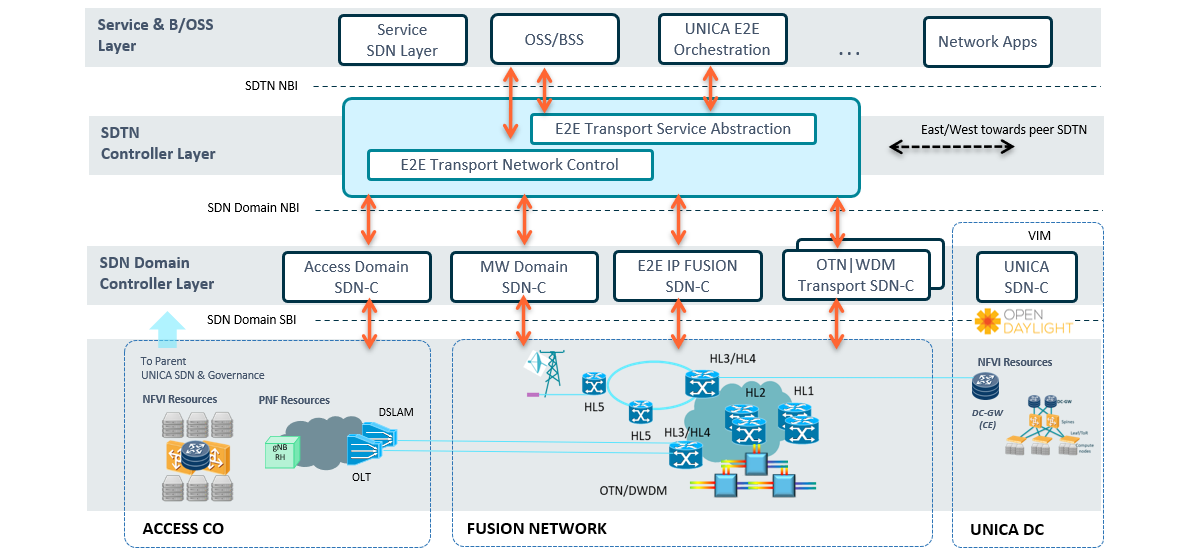
\includegraphics[scale=1]{figs/ifusion_architecture.png}
	\caption{iFUSION architecture}
	\label{FIG:1}
\end{figure*}

The key elements of the SDN iFUSION architecture are the following:

\begin{itemize}
\item \textbf{SDN Domain}: It is a set of network elements under the supervision of the same SDN Controller. There are several possible levels in the decoupling of control and data planes. The preferred level of decoupling in Telefonica depends on the network technology. For example, in the case of MPLS, the network element runs the distributed protocols (e.g. IS-IS TE, RSVP-TE) and the controller only needs to configure it.

\item \textbf{SDN Transport}: It is the whole network controlled by following SDN principles. It is divided into SDN Domains for technology/scalability/administrative principles. A SDN Transport Controller (also referred as SDN Orchestrator), will take care of stitching the different domains/layers/technologies.

\item \textbf{SDN Domain Controller}: This element is in charge of a set of network elements. It has standard southbound interfaces that depend on the technology, but not in the equipment vendor, to communicate with the network elements. It also has a northbound interface to communicate with the SDN Orchestrator and the OSS.

\item \textbf{Software Defined Transport Network (SDTN) Controller}: In case several SDN Domains are needed, the SDN Transport Controller is in charge of providing services through several domains. 

\item \textbf{Southbound Interface}: It is the interface, based on a standard, between the SDN Domain Controller and the Network Element. Not only the communication protocol needs to be standard, but also the data model used.

\item \textbf{Northbound Interface}: If is the interface, based on a standard, between the SDN Domain Controller and the OSSs and SDN Transport.

\item \textbf{Service SDN controller}: An additional SDN layer that takes into account services might be needed. 
\end{itemize}

The iFUSION architecture is designed as a hierarchical model where each network segment is controlled by a dedicated SDN Domain controller. The transport network, due to its wide scope and complexity, is divided in three main technology domains: \hyperref[section:ip]{IP}, \hyperref[section:mw]{Microwave} for wireless transport, and \hyperref[section:dwdm]{Optical} for transmission. 

The Software Defined Transport Network (SDTN) Controller is responsible to orchestrate the respective SDN Domain controllers within the transport segment (IP, Optical and MW) through the Domain Controllers\'NBI, providing an end-to-end transport network vision. The SDTN Controller aggregates demands from the management and services layer exposing a unified NBI which should provide resource configuration abstraction and technology agnostic service definition. 

The SDTN entails the following functions: 
\begin{enumerate}
    \item End-to-end service binding and mapping.
    \item End-to-end Transport Service Abstraction.
    \item End-to-end resource/topology discovery and composition.
    \item End-to-end resource visualization.
\end{enumerate}

The SDN Domain controllers, on the other hand, are in charge of all the devices in the domain. Each SDN Domain controller unifies the device configuration interface and provides vendor-agnostic network configuration, monitoring and resource discovery. Besides, the Domain Controller exposes high-level network services abstraction to OSS and BSS layers through its North Bound Interface (NBI). Therefore, the abstraction of device specific configuration from network service definition is one of the main features that the SDN controller implements. Moreover, the SDN Domain Controllers entail the function of Path Computation Element to manage and optimize traffic engineering in the domain.

\subsection {IP domain}
\label{section:ip}
IP networks are deployed following a hierarchical model, mixing equipment from different vendors. The IP boxes are interoperable at data plane level and control plane level (e.g. routing protocols such as IS-IS, OSPF or BGP). Due to scalability reasons, the IP networks are typically subdivided in IP domains, so the routing and control protocols are confined to their respective domains.

The foreseen SDN solution for IP segment is based on a single, multi-vendor IP SDN Domain Controller in charge of configuring the IP network elements, as shown in \ref{FIG:2}.

\begin{figure*}
	\centering
		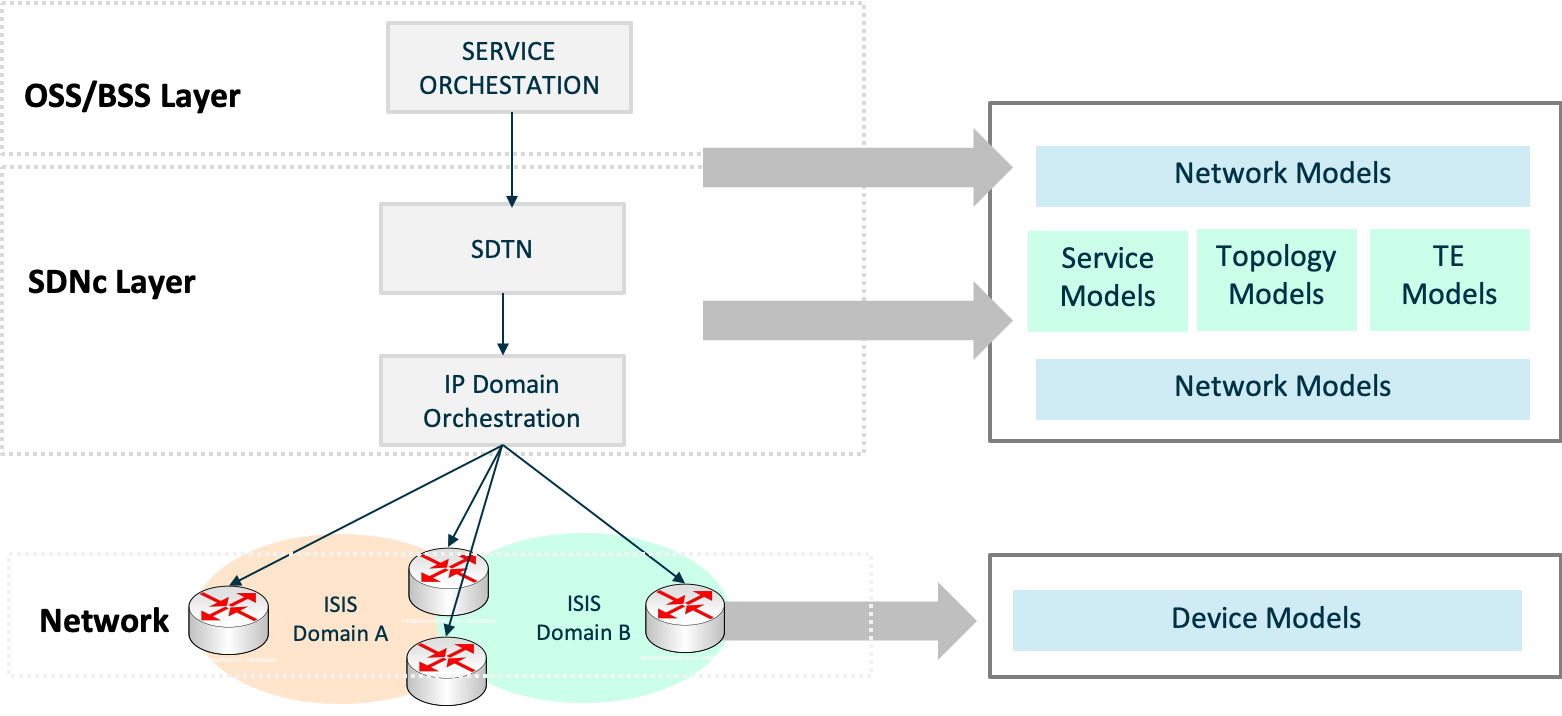
\includegraphics[scale=1]{figs/ifusion_multidomain_2.png}
	\caption{Single multi-vendor IP SDN Domain Controller deployment}
	\label{FIG:2}
\end{figure*}

The target SBI for vendor agnostic device configuration shall be compliant with NETCONF \cite{enns2011network} standard protocol. The  set of device configuration data models (SBI) for the IP segment is still under definition but shall be defined in YANG \cite{bjorklund2016yang} modelling language, while it could be inherit or complemented from/by other alternative modelling tools, such UML, to help its definition.

From the implementation perspective, it is assumed that devices might not natively support the data models selected, and thus a mediation layer could be required to be implemented between the controller and the devices. Such a mediation layer would be considered as an interim solution and, if present, shall be transparent without impacting on the performance and capabilities of the defined interface. 

Additionally to pure device configuration, the IP SDN Domain controller shall perform Traffic Engineering and Path Computation. With that purpose, some standard and mature control protocols such PCEP and BGP-LS for MPLS networks, shall be implemented to complete the definition of the SBI. As a result, Telefonica expects that the IP SDN controller will assume the control/management of:
\begin{itemize}
\item Device configuration of interfaces (VLANs) and routing protocols (BGP, ISIS…)
\item Traffic Engineering of MPLS tunnels (LSPs). 
\item Overlay networks services (L2/L3 VPNs) device configuration (VRFs,\dots)
\end{itemize}

The IP SDN Domain controller will be the main entry point to the network elements, to avoid overloading the elements and providing a coherent view. The NBI of the controller will also be based on standard models defined in YANG and implemented either on NETCONF or on its lightweight version RESTCONF \cite{bierman2017restconf} with XML/JSON encoding. The NBI shall provide to higher entities within the SDN hierarchy:
\begin{itemize}
\item Device inventory information.
\item A layered topology view (L2/L3, MPLS) of its controlled network entities.
\item LSPs provisioning and path computation.
\item Device abstraction for network services towards the SDTN Controller, i.e., for overlay services VPNs (L2, L3)
\item Network state and performance monitoring information of the IP domain. 
Apart from the previous network segments, SDN will also be introduced in other network environments related with Virtualization and the evolution of the Central Offices.
\end{itemize}

\subsection{Optical domain}
\label{section:dwdm}
Transport WDM networks from different system vendors are deployed on a regional basis, either for technology redundancy, due to different optical performance requirements (metro vs. long-haul), or simply for commercial reasons. 

Without line-side interoperability of the different WDM transceivers and Reconfigurable Optical Add-Drop Multiplexers (ROADMs), there is not a competitive advantage on a uniform configuration interface of the optical devices, since they cannot neither be mixed in a multi-vendor scenario, due to the fact that both line systems and transceivers must be from the same vendor.

With this in mind, in the short term, Optical SDN controllers are expected to provide network programmability and interoperability towards upper layers (multi-layer) and between vendors (multi-domain, multi-vendor) through the support of standard NBIs (i.e. coordination will be provided by upper layer hierarchical SDN controller). This short term approach will enable the setup and tear down of connections in optical channels (OCh and ODU layers), the discovery the network resources to compose a layered uniform view based on the OTN hierarchy, and the monitoring of the optical network. 

The SDN architecture proposed is compatible with a legacy control scenario where a distributed GMPLS control plane has been already deployed. GMPLS control plane can be centrally managed by a SDN domain controller by well-know and mature control protocols, such as PCEP, OSPF and/or BGP-LS already supported in GMPLS devices, beneficing the gradual introduction of SDN. However, current NMS solutions shall evolve to, or co-exist with, the SDN Controller model, enabling network programmability through its NBIs while keeping the current offered features for network creation, resources discovery and monitoring and service creation for L0/L1 layers. Standardization efforts targeting the definition of standard NBIs that can facilitate multi-vendor interoperability (by maintaining administrative domains for each vendor) such as ONF Transport API (T-API) [11] and IETF models [12] are the more promising definitions to implement such capabilities by abstracting the specific configuration of current distributed control planes embedded in Automatic Switched Optical Network (ASON) architectures. 
iFUSION relays on ONF Transport API 2.0 as as the reference NBI for the SDN implementation in the optical transport segment, having been experimented in several proof of concepts [15]. 

In the medium and long term, the direct programmability of the components can have interest in Point-To-Point, Metro and Regional scenarios, where disaggregation of optical transceivers and line side components can play an important role. In this line, OpenROADM [12] and OpenConfig [13] projects have already defined device configuration models for transponders and open line systems. Telefonica is approaching this transformation of the optical control in two phases:

\begin{enumerate}
    \item Partial disaggregation, as a medium term objective, where the target is to define a standard interface based on NETCONF/YANG, which allows of the Optical SDN Controller to manage third-party terminal devices (i.e., transponders) that can transmit over the vendor line system.
    
    \item Full disaggregation, in the long term, where the objective is the open management of the line system, i.e., the defragmentation of the optical transport network in vendor islands by the adoption of a common standardized interface for open line systems (multi-vendor) to be managed by a single optical SDN Controller.
\end{enumerate}

\subsection{Wireless transport domain}
\label{section:mw}
Wireless Transport networks, typically consisting on microwave (MW) radio links, are deployed on a point-to-point basis covering a given region using several vendors. Currently the wireless networks are operated through vendor proprietary Network Management Systems (NMS) with specific proprietary interfaces.

Operation, configuration and maintenance activities are performed manually and statically. Furthermore, this diversity in NMSs and vendor installed base prevents from using advanced applications that could provide more sophisticated features (e.g. power management or multi-layer coordination [14]), since actual integration costs disincentive any effort in such direction. 

This reality has fostered the standardization of a common framework [15] for definition of a unified and standard control plane for microwave systems, pursuing as objective the multi-vendor interworking, multi-layer control, and network-wide coordination.
For practical SDN deployments in this technical domain the ONF has released a standard model published as TR-532 document [16], with the support of the wide community of MW system manufacturers. A number of PoCs have served as validation steps of the viability of the model, as well as helping to refine it and to prepare the industry for this evolution. This is the data model adopted by Telefonica in the iFUSION architecture.

The proposed model is aligned with the view of the SDN Domain Controller as a vendor-agnostic configurator of the MW network. It leaves the service definition to upper applications which need to provide the intelligence to deploy and manage end-to-end services, by configuring every device involved individually through the SDN controller.

Interestingly, one of the outcomes of these PoC has been the definition of a Mediator, in principle devoted to experiment with the model, but later on identified as a mean of integrating legacy MW systems with an evolved SDN-based deployment, then protecting investments and ensuring smooth transition towards SDN.  

\subsection{Integration of SDTN in the overall operator’s systems architecture}
\label{section:sdtn}
The SDTN Controller will keep visibility of all the transport network segments. It will expose an abstracted topology view of the network resources and the available set of network services to different clients through its North-Bound APIs.  
One of the main drivers of deploying an SDTN controller is service automation. SDTN will enable it, progressively, facilitating that services and network configurations carried out manually today become automated and available through this abstraction layer.  The level of abstraction can be different according to the needs of the northbound client (e.g. OSS, service orchestrators/SDN controllers, NFV orchestrator, etc.). 

The information exported through the NBI towards OSS and other platforms will cover progressively a number of functional areas. The service’s provisioning within the Resource Lifecycle Management (RLM) domain will be the first set of functionalities adopted by the SDTN controller, which will progressively include Performance Management (PM) and Network Planning and Design (NPD), and finally Fault Management (FM) and Resource Inventory Management (RIM) areas which includes the major vendor specific management information will be included in the SDTN. The inclusion of these functional blocks is conditioned to the standardization of the required data models for the SDTN NBI and SDN Domain controllers SBI. 

On the SBI of the SDTN, each technology Transport Domain SDN Controller shall expose vendor agnostic network level programmability and resource discovery functionalities. The SDTN Controller SBI is intended, but not limited, to provide access to device’s configuration data, to expose per-OSI layer topology and network inventory information, and to offer active monitoring of device configuration changes and network state data (i.e., traffic statistics). Alarm and device inventory information for FM and RIM respectively, is intended to be managed at the SDN Domain controllers in a first phase, but its exposure through the SDTN will be evaluated too.


\section{Network Programmability - TEF gCTIO}
\label{section:net}

\section{Service Models - TEF gCTIO}
\label{section:models}

\subsection{IP Network Models}

\subsubsection{L3NM}

The Layer 3 Virtual Private Network (VPN) service defined in RFC 4364 \cite{rosen2006rfc} provides a multipoint, routed service to the customer over an IP/MPLS core. The L3VPNs are widely used to deploy 3G/4G, fixed and enterprise services principally due to the fact that not only several traffic discrimination policies can be applied to transport and guarantee SLAs across the network but also because several stitching methodologies can be applied to combine access and transport services. 

Some service models has been defined and standardized until now. L3SM \cite{rfc8299} is a Customer Service Model that describes the requirements of a L3VPN service from the point of view of the customer. It defines a YANG data model that can be used in the communication between customers and network operators. 

L3NM is a Service Network Model \cite{voyer2019internet}. The L3NM YANG model is exposed by network controllers to manage and control the VPN Service configuration. The model describes a VPN Service in the service provider network. It contains information of the service provider network such as NE-ID and Interfaces-ID and might include allocated resources such as the Route Targets and Route Distinguishers.

The L3NM model is Network Centric, it is focused on the service provider internal network parameters. The data model can be used to facilitate communication between the service orchestrator and the SDTN network controller. Also, the SDTN network controller can further include network specific information in the service request (i.e. transport LSP binding, Router Targets assignation, routing profiles or encryption). In addition, it facilitates multi-domain orchestration, where logical resources (such as route targets or route distinguishers) must be synchronized between domains.
The L3NM model does not keep any of the commercial customer parameters, which belong to the OSS/BSS layer.

\begin{figure}
	\centering
		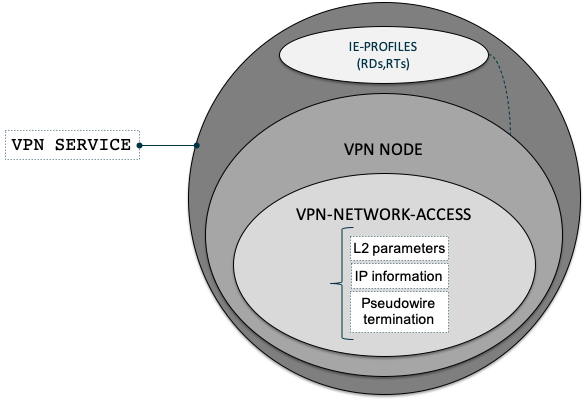
\includegraphics[scale=0.35]{figs/L3NM.png}
	\caption{L3NM Data model structure}
	\label{FIG:l3nm}
\end{figure}

\begin{lstlisting}[basicstyle=\ttfamily\small,label=l3nm,caption=L3NM Yang Structure]
module: ietf-l3vpn-ntw
 +--rw l3vpn-ntw
  +--rw vpn-profiles
  |  ...
  +--rw vpn-services
   +--rw vpn-service* [vpn-id]
      +--rw vpn-id                  l3vpn-svc:svc-id
      +  ...
       +--rw vpn-node* [ne-id]
          +--rw ne-id                      string
          + ...
          +--rw vpn-network-accesses
          |  +--rw vpn-network-access* [id]
\end{lstlisting}

\subsubsection{L2NM}

\subsubsection{Network Topology}

The proposed control architecture relies on providing different levels of abstraction for each control layer. Therefore, the needs in terms of topology and knowledge of the service provider network differ among components.

\subsection{Optical Network Model - TEF gCTIO}

\subsubsection{Provisioning}

\subsubsection{Topology}

\subsection{End-to-end Use Cases Definition}
We have defined two end-to-end uses cases as follows in the next subsections:

\subsubsection{Multi-domain IP L3VPN provisioning}
The IP L3VPN service defined in RFC4364 \cite{rfc4364} provides a multipoint, routed service to the customer over an IP/MPLS core. The L3VPNs are widely used to deploy 3G/4G, fixed and enterprise services principally due to the fact that several traffic discrimination policies can be applied in the network to transport and guarantee the right SLAs to the mobile customers.

The purpose of this use case is to describe the Telefonica’s reference NBI for the multi-domain IP L3VPN provision based on the interactions with IP SDN-Cs, including the information models which conforms this interface. The scope includes multiple domains within the same network, where each SDN-C is required to implement the IETF L3NM model described in subsection 4.1.1. We assume an upper OSS send a provisioning query for a IP L3VPN,  that goes through intermediatation of the SDTN, which orchestrates the provision of the service and expose an unified view of it.

Notice that the Multi-domain L3VPN Service can only be exposed if there are links interconnecting all the different network domains over which the service would be passing through. Where the Multilayer Topology use case will be explained in further detail in the next chapter. 

From a signalling perspective, it is required that every origin PE-Routers from a region, usually concentrated in an upper layer, can establish an end-to-end LSP to the destination PE-Router. Networks is organised by clusters and rings within. Every cluster is closed from a connectivity perspective by clusters/ring heads. Those Head-Routers have the Autonomous System Border Router (ASBR) role as well as Inline Router reflector for its Region/Cluster. 

Thus, to forward the traffic from the L3VPN services, the ASBR routers from each region establish an eBGP session against the Core-Routers. This session exports the Router-ID plus Label information of all the routers in the region using BGP-LU \cite{rfc8277}. Additionally, there is another eBGP session between the HL3 of the region and the core Router-Reflectors to export the VPNv4 routes from each VPN service. This eBGP session requires a mandatory a Next-Hop-Unchanged configuration to avoid network loops or misconfigured paths. All of this control plane setup allows the creation of an end-to-end LSP from the access layer to the platforms without changing the configuration during the service provisioning.

Additionally, to deploy any of this service the network has to fulfill the following basic requirements established between origin and destination:
\begin{itemize}
    \item IGP Router-ID/Loopback connectivity.
    \item MPLS and Labelling mechanism LDP, RVSP, other. 
    \item MP-BGP (family vpnv4/6, ipv4/6).
    \item Virtual Routing network instance. 
\end{itemize}

In our proposal solution, Multidomain IP L3VPN Provision fulfill connectivity and SLAs compliance between sites using a common infrastructure, support changes in topology as well as in L3VPN parameters such as scheduler and QoS profile. 

The interface between the SDTN and SDN-C shall integrate only mandatory information that is held at the OSS layer or that is requested by the customer service. For this specific use case, the parameters and request will have the following four steps per each domain. Fig.  ~\ref{FIG:multidomain_service_provisioning_workflow} depicts the corresponding workflow where the following steps are needed to provision the multi-domain service:
\begin{enumerate}
    \item Create Site (VPN.L3.Site.Add)
    \item Create Bearer (VPN.L3.Bearer.Add)
    \item Create VPN (VPN.L3.Add)
    \item Create Access (VPN.L3.Access.Add)
\end{enumerate}

\begin{figure}
	\centering
		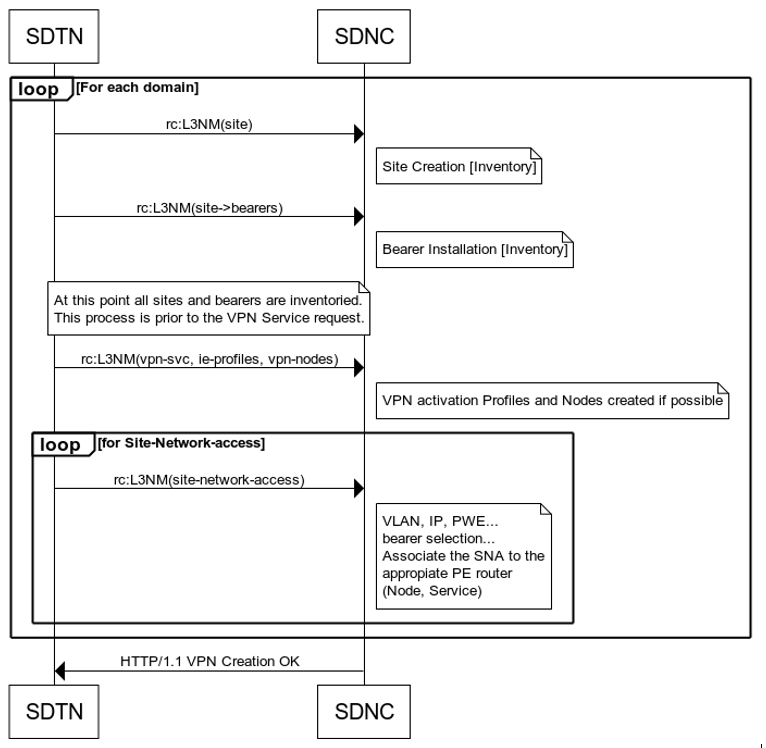
\includegraphics[width=\linewidth]{figs/multidomain_service_provisioning_workflow.png}
	\caption{Workflow for multi-domain service provisioning SDTN-SDN-C}
	\label{FIG:multidomain_service_provisioning_workflow}
\end{figure}

\subsubsection{Multi-layer Topology}
The multi-layer topology use case is based on the perspectives provided by all the IP and Optical WDM/OTN SDN-Cs. The scope of it, includes multiple domains within the same network, where each SDN-C will export its IETF context or T-API context, correspondingly. Use case is built upon the ONF T-API \footnote{https://wiki.opennetworking.org/display/OTCC/TAPI} Topology module and Connectivity Service module for L2-L0 Optical side, IETF implementations, specifically IETF RFC8345 \cite{rfc8345} as basis for the generic network model, and a reduced version of YANG Data Model for Traffic Engineering in \cite{ietf-teas-yang-te-topo-22} for L1 IP topology augmenting the generic model. We have built a new model putting all together following the best practices defined in previous works in the topic. In order to provide an explicit multi-layer topology representation of the whole network for all its layers. 

A multi-layer multi-domain topology abstraction unified view is required for vendor-agnostic integration on Service Providers systems. We propose to create a unique topology based on the T-API Topology and IETF Topology Flat Abstraction models which collapses all layers. A key element to achieved that, it is the usage of a correlation plug-id concept, to join the IP and Optical layers. Due to there is no a dynamic protocol or common element between the ONF/IETF standards that would allow their correlation. 

There are some pre-requisites to build the multi-layer topology and those are:
\begin{itemize}
    \item The context of the optical layer topology MUST already be known by the SDTN controller.
    \item The context of optical services MUST be known by the SDTN controller.
    \item The context of the IP layer topology MUST be already known by the SDTN controller.
\end{itemize}

The SBI for this use case base in the IP part representation is supported on the RFC8345. In this RFC, a basic network representation is done using an abstract network model (“ietf-network”) with the set of parameters described in the (4.1.3 subsection). These parameters are common for all the networks described in this document (L1, L2, L3, and UNI), by means of augmentation.  

Our detail proposal as follows: 

In the RFC8345 (generic network) it’s considered to use the supporting-termination-point through the
\\ \textit{ietf-network:termination-point={tp-id}} attribute.

\begin{lstlisting}[basicstyle=\ttfamily\small,label=tps,caption=Supporting termination point Structure]
/nw:networks/nw:network/nw:node:
    +--rw termination-point* [tp-id]
    +--rw tp-id 
    +--rw supporting-termination-point
       +--rw network-ref
       +--rw node-ref
       +--rw tp-ref
\end{lstlisting}

Where the supporting-termination-point represents another termination point in an underlay network. Considering this, the list of attributes will show the next information: 
\begin{itemize}
    \item The \textit{network-ref} references an underlay network, where the supporting Network for this case specifically must be \textbf{l1-topology}.
    \item \textit{Node-ref} represents a node in an underlay network, where the supporting node name must be the node-id in the \textbf{l1-topology}.
    \item \textit{Tp-ref} references the underlay terminal point itself. The supporting termination point must be \textit{tp-id} in the in the \textbf{l1-topology}.
\end{itemize}


Finally, for the construction of the multi-layer topology, it is necessary to perform the process by layers satisfying the prerequisites, in which the SDTN will perform the task of correlating the values that until now will be filled manually in the plug-id attributes in IP and Optical layers. The process proposed is depicted as workflow in Fig. ~\ref{FIG:topology_workflow}.

\begin{figure}
	\centering
		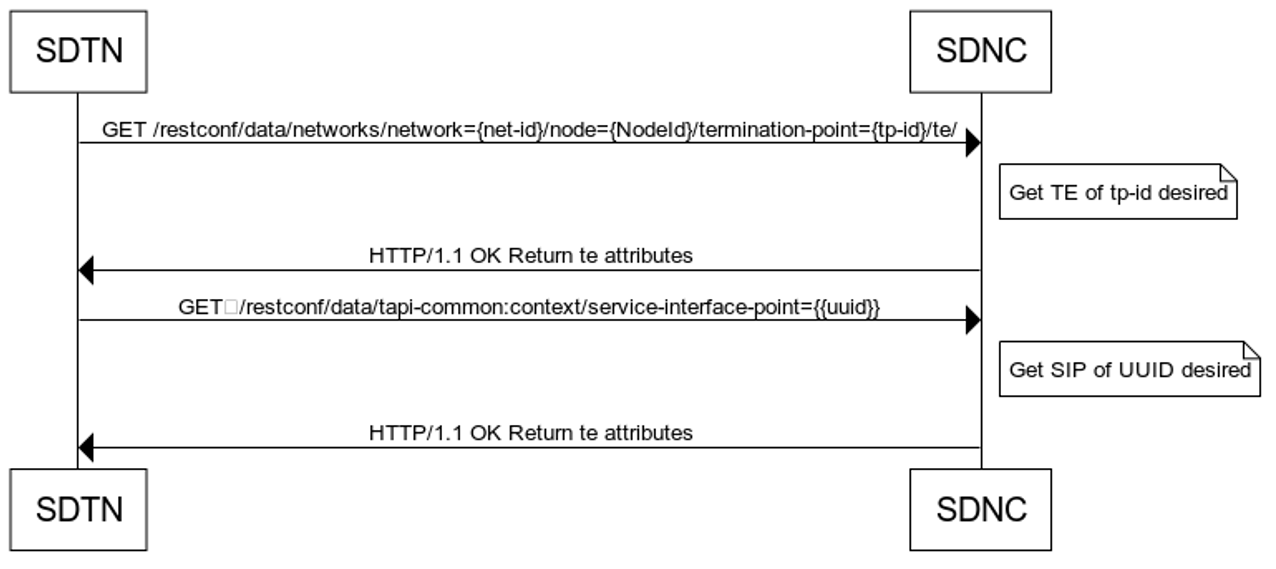
\includegraphics[width=\linewidth]{figs/topology_workflow.png}
	\caption{Workflow for multi-layer topology SDTN-SDN-C}
	\label{FIG:topology_workflow}
\end{figure}


\begin{figure*}
	\centering
		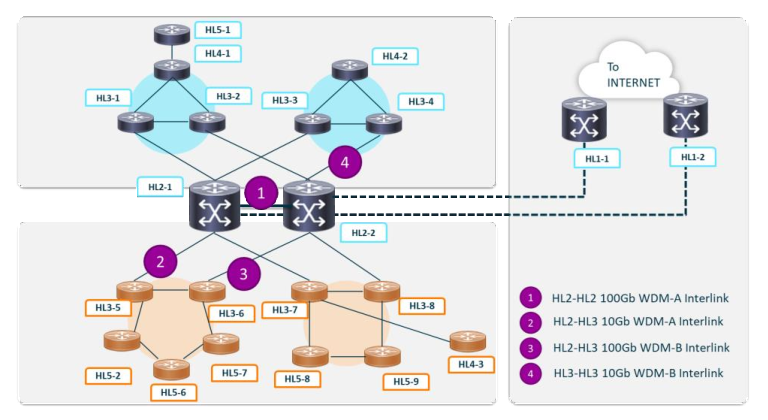
\includegraphics[scale=1]{figs/field_trial_environment_ip.pdf}
	\caption{Network Plane of the Field Trial Environment for IP/MPLS Testing and Evaluation}
	\label{FIG:field_trial_ip}
\end{figure*}

\begin{figure*}
	\centering
		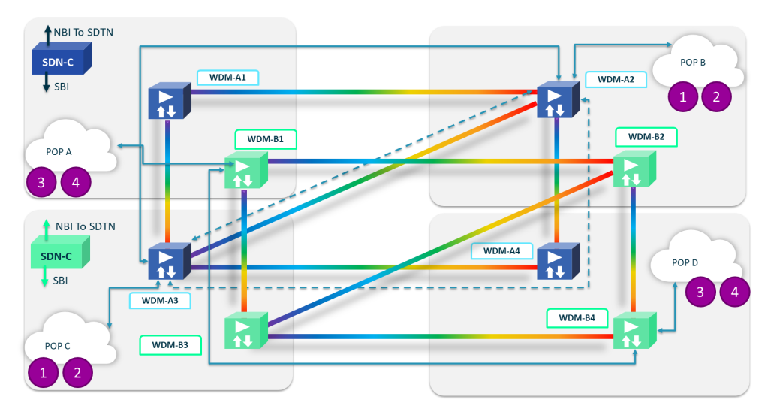
\includegraphics[scale=1]{figs/field_trial_environment_optical.pdf}
	\caption{Network Plane of the Field Trial Environment for Optical/WDM Testing and Evaluation}
	\label{FIG:field_trial_optical}
\end{figure*}

\section{Field Trial Environment for iFusion SDTN Demonstration}
\label{section:trial}

We have deployed a field trial environment for demonstrating, testing and evaluating the end-to-end multi-domain cases and the SDN-based iFusion Architecture. We describe the two main layers which compose the field trial. Fistly, a \textit{Control Layer} is comprised of two SDN IP Domain Controllers for a multivendor IP/MPLS network using as underlying WDM infrastructure and working in parallel with two SDN Optical Domain Controllers. On top of that, a multilayer multidomain SDTN Controller is orchestrating the uses cases. Secondly, the \textit{Network Layer} is comprised of a Metropolitan WDM Network with nx100Gb Lambda capacity providing interlink capabilities for a multidomain IP/MPLS network following a hierarchical architecture that we denominate from HL1 (Hierarchical Layer No. 1) to HL5. We detail each of the layers in the next subsections. 

\subsection{Control Layer}
A hierarchical SDTN architecture is built upon the reference design guidelines described in Section 2. Infinera Trascend Maestro\footnote{https://www.infinera.com/solutions/intelligent-automation/}, acting as SDTN controller, orchestrates four (4) SDN-C one for each domain.
From the IP control perspective, SDN-Cs communicate with NEs via NETCONF/YANG with the OpenConfig data models and RESTconf with SDTN. As explained in Section 4.3.1, we have extended the end-to-end signalling building a seamless MPLS multi-domain IP/MPLS network. In other hand, from the Optical perspective, SDN-Cs follow a similar integration. At SBI, OpenROADM + OPenConfig models are used on top of NETconf/YANG protocol. At NBI, a T-API implementation is used.  

\subsection{Network Layer}
We use a scale representation in terms of quantity of equipment but a full network field trial with all the hierarchical layers that compose a Service Provider real deployment. In our notation and architecture the IP/MPLS-base network is comprised of five (5) layer with the following responsibilities: 
\begin{itemize}
    \item HL1: Core P/PE-Routers acting as Toll Gates for interconnection the Service Provider to the International Exit and using eBGP logical structure for publishing public IPv4/IPv6 prefixes to IP gates from and to a Tier-1/2 international Internet provider.
    \item HL2: Core P-Router responsible for the transportation of traffic between main cities and metropolitan areas sending/receiving traffic to HL1 interconnections from/to the International Internet.
    \item HL3: PE-Routers responsible for the aggregation and conglomeration of traffic from metropolitan and regional areas coming from network clusters and rings covering main and secondary cities for both fixed and mobile services.
    \item HL4: PE-Routers able to collect traffic from fixed access networks (DSLAM/CMTS/OLT) in metropolitan areas and high capacity corporate services. And to collect traffic from mobile access networks coming from HL5 (former cell-site routers) for all generations 2G/3G/4G, 4.5G and new 5G in the near future.
    \item HL5: Provides connectivity access to corporations, enterprises, small businesses and mobile terminal nodes (BTS, NodeB, eNodeB) in remote areas. Formerly known as cell site routers in Mobile Service Providers, but now evolved and converged to serve multiple fixed plus mobile segments.     
\end{itemize}

Four (4) IP/MPLS-based network links are transported by a two-vendor WDM underlying infrastructure. Fig. ~\ref{FIG:field_trial_ip} depicts in purple the four interlinks 2x100Gb and 2x10Gb.  

Regarding the optical transport infrastructure, we have built a dual-plane independent metropolitan WDM networks. Comprised of a ring of (4) four nodes each with nx100Gb and nx10Gb lambda capacity. Fig. ~\ref{FIG:field_trial_ip} illustrates the optical WDM part of the field trial enviroment.


\section{Results  - TEF COL}
\label{section:results}

Con las trazas sería suficiente podemos elaborarlo luego.

\subsection{Single-domain L2VPN provisioning}

\subsection{Multi-domain IP L3VPN provisioning}

\subsection{Multi-layer Topology Visualization}

\section{Conclusions}
\label{section:conclusions}

\printcredits

%% Loading bibliography style file
%\bibliographystyle{model1-num-names}
\bibliographystyle{cas-model2-names}

% Loading bibliography database
\bibliography{bibliography}


%\vskip3pt

\bio{figs/1010179793S.jpg}
Phd Candidate.
\endbio

\bio{}
Author biography with author photo.
\endbio

\bio{}
Author biography with author photo.
\endbio

\end{document}

